\documentclass[border=5pt]{standalone}
% Shared by every figure. Colour marks the TYPE of a quantity, never decoration:
%   blue   (vec) equivariant: rotates with its fragment     -- solid arrows
%   orange (inv) invariant: unchanged by any rotation        -- dashed arrows
%   aqua   (att) attention / communication between elements
%   violet (out) what the network outputs
% Text is always ink; a coloured mark next to it carries the meaning.
\usepackage{amsmath,amssymb,bm}
\usepackage{tikz}
\usetikzlibrary{arrows.meta,positioning,fit,backgrounds,calc,shapes.geometric,
  shapes.misc,decorations.pathreplacing,decorations.pathmorphing,matrix,
  patterns,cd,shadows}
\definecolor{vec}{HTML}{2A78D6}
\definecolor{inv}{HTML}{EB6834}
\definecolor{att}{HTML}{1BAF7A}
\definecolor{out}{HTML}{4A3AA7}
\definecolor{ink}{HTML}{0B0B0B}
\definecolor{ink2}{HTML}{52514E}
\definecolor{ink3}{HTML}{8A877F}
\definecolor{neutral}{HTML}{F0EFEC}
\definecolor{rule}{HTML}{CFCCC4}
\definecolor{pieceA}{HTML}{E4E1DA}
\definecolor{pieceB}{HTML}{CDC9BF}
\definecolor{pieceC}{HTML}{B3AEA2}
\colorlet{vecfill}{vec!9}
\colorlet{invfill}{inv!10}
\colorlet{attfill}{att!11}
\colorlet{outfill}{out!9}
\tikzset{
  >={Stealth[length=2.3mm,width=1.7mm]},
  every picture/.style={line cap=round, line join=round},
  box/.style={draw=ink2, fill=neutral, rounded corners=2.5pt, align=center,
    font=\small, inner sep=4pt, minimum height=8mm, text=ink, line width=0.6pt, nohyph},
  vecbox/.style={box, draw=vec, fill=vecfill},
  invbox/.style={box, draw=inv, fill=invfill},
  attbox/.style={box, draw=att, fill=attfill},
  outbox/.style={box, draw=out, fill=outfill},
  plain/.style={box, draw=ink3, fill=white},
  arr/.style={->, draw=ink2, line width=0.7pt},
  vecarr/.style={->, draw=vec, line width=1.1pt},
  invarr/.style={->, draw=inv, line width=1.1pt, dash pattern=on 3.2pt off 1.8pt},
  attarr/.style={->, draw=att, line width=1.1pt, dash pattern=on 1.2pt off 1.4pt},
  outarr/.style={->, draw=out, line width=1.1pt},
  nohyph/.style={execute at begin node={\hyphenpenalty=10000\exhyphenpenalty=10000\relax}},
  lbl/.style={font=\footnotesize, text=ink2, align=center, nohyph},
  tlbl/.style={font=\footnotesize, text=ink, align=center, nohyph},
  group/.style={draw=ink3, dashed, rounded corners=5pt, inner sep=7pt},
  op/.style={circle, draw=ink2, fill=white, inner sep=0pt, minimum size=5.2mm,
    font=\small, line width=0.6pt},
  piece/.style={fill=#1, draw=none},
  intact/.style={draw=ink2, line width=0.6pt},
  fracture/.style={draw=ink, line width=1.5pt},
  token/.style={circle, fill=att, draw=white, line width=0.5pt, inner sep=0pt,
    minimum size=4.2pt},
  vtx/.style={circle, fill=ink, inner sep=0pt, minimum size=3pt},
  panel/.style={font=\small\bfseries, text=ink, anchor=north west},
}
% one piece of the cartoon, in its own centred frame: fill, intact edge, fracture edge
\newcommand{\drawpiece}[2]{% #1 = A|B|C, #2 = fill colour
  \fill[#2] \csname Piece#1\endcsname;
  \draw[intact] \csname Intact#1\endcsname;
  \draw[fracture] \csname Crack#1\endcsname;}
% a legend entry: a short line in a given style, then its text
\newcommand{\legendline}[3]{% #1 position, #2 style, #3 text
  \draw[#2] (#1) -- ++(0.7,0) node[right, tlbl, text=ink] {#3};}

\begin{document}
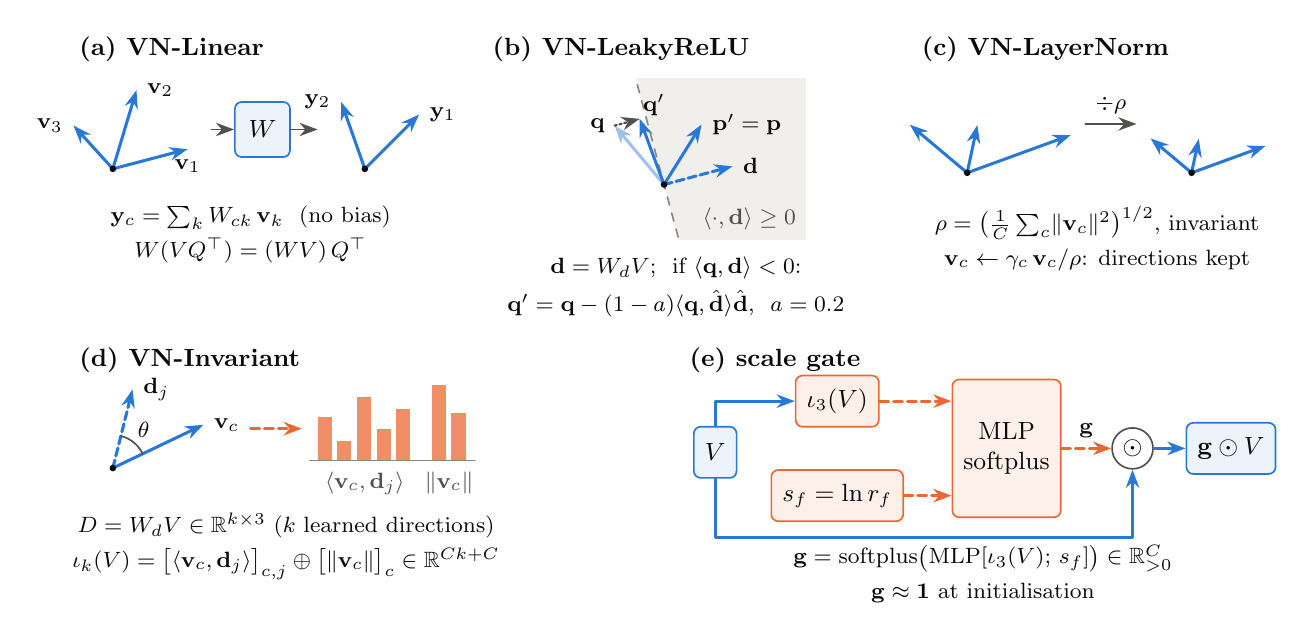
\begin{tikzpicture}
  \tikzset{form/.style={lbl, text=ink, anchor=north}}
  % ======================= (a) VN-Linear =======================
  \begin{scope}[shift={(0,0)}]
    \node[panel] at (0,1.95) {(a) VN-Linear};
    \coordinate (o1) at (0.55,0.15);
    \draw[vecarr] (o1) -- ++(0.95,0.25) node[below, tlbl] {$\mathbf v_1$};
    \draw[vecarr] (o1) -- ++(0.3,1.0) node[right, tlbl] {$\mathbf v_2$};
    \draw[vecarr] (o1) -- ++(-0.5,0.55) node[left, tlbl] {$\mathbf v_3$};
    \fill[ink] (o1) circle (1.2pt);
    \node[vecbox, minimum height=7mm, minimum width=7mm] (W) at (2.45,0.65) {$W$};
    \draw[arr] (1.8,0.65) -- (W.west);
    \draw[arr] (W.east) -- (3.15,0.65);
    \coordinate (o2) at (3.75,0.15);
    \draw[vecarr] (o2) -- ++(0.69,0.69) node[right, tlbl] {$\mathbf y_1$};
    \draw[vecarr] (o2) -- ++(-0.3,0.85) node[left, tlbl] {$\mathbf y_2$};
    \fill[ink] (o2) circle (1.2pt);
    \node[form] at (2.3,-0.2) {$\mathbf y_c=\sum_k W_{ck}\,\mathbf v_k$\ \ (no bias)\\[3pt]
      $W(VQ^{\top})=(WV)\,Q^{\top}$};
  \end{scope}

  % ======================= (b) VN-LeakyReLU =======================
  \begin{scope}[shift={(5.25,0)}]
    \node[panel] at (0,1.95) {(b) VN-LeakyReLU};
    \coordinate (o) at (2.3,-0.05);
    \begin{scope}
      \clip (0.85,-0.75) rectangle (4.1,1.3);
      \fill[neutral] ($(o)+(105:3)$) -- ($(o)+(-75:3)$) -- ++(15:4) -- ++(105:6) -- cycle;
      \draw[ink3, dashed, line width=0.6pt] ($(o)+(105:3)$) -- ($(o)+(-75:3)$);
    \end{scope}
    \node[lbl, anchor=south east] at (4.1,-0.75) {$\langle\cdot,\mathbf d\rangle\ge 0$};
    \draw[vecarr, dash pattern=on 3pt off 1.5pt] (o) -- ++(15:0.9) node[right, tlbl] {$\mathbf d$};
    \draw[vecarr] (o) -- ++(58:0.9) node[right, tlbl] {$\mathbf p'=\mathbf p$};
    \draw[vec!45, line width=1.1pt, ->] (o) -- ++(-0.628,0.749) coordinate (q);
    \node[tlbl, anchor=east] at (q) {$\mathbf q$};
    \draw[vecarr] (o) -- ++(-0.309,0.835) coordinate (qq);
    \node[tlbl, anchor=south west, inner sep=1pt] at (qq) {$\mathbf q'$};
    \draw[ink2, densely dotted, line width=0.8pt, ->] (q) -- (qq);
    \fill[ink] (o) circle (1.2pt);
    \node[form] at (2.45,-0.85) {$\mathbf d=W_dV$; \ if $\langle\mathbf q,\mathbf d\rangle<0$:\\[3pt]
      $\mathbf q'=\mathbf q-(1-a)\langle\mathbf q,\hat{\mathbf d}\rangle\hat{\mathbf d}$, \ $a=0.2$};
  \end{scope}

  % ======================= (c) VN-LayerNorm =======================
  \begin{scope}[shift={(10.7,0)}]
    \node[panel] at (0,1.95) {(c) VN-LayerNorm};
    \coordinate (o3) at (0.7,0.1);
    \draw[vecarr] (o3) -- ++(20:1.4);
    \draw[vecarr] (o3) -- ++(78:0.62);
    \draw[vecarr] (o3) -- ++(140:0.95);
    \fill[ink] (o3) circle (1.2pt);
    \draw[arr] (2.2,0.72) -- node[above, tlbl] {$\div\rho$} (2.85,0.72);
    \coordinate (o4) at (3.55,0.1);
    \draw[vecarr] (o4) -- ++(20:1.0);
    \draw[vecarr] (o4) -- ++(78:0.44);
    \draw[vecarr] (o4) -- ++(140:0.68);
    \fill[ink] (o4) circle (1.2pt);
    \node[form] at (2.35,-0.2) {$\rho=\big(\tfrac1C\sum_c\lVert\mathbf v_c\rVert^2\big)^{1/2}$, invariant\\[3pt]
      $\mathbf v_c\leftarrow\gamma_c\,\mathbf v_c/\rho$: directions kept};
  \end{scope}

  % ======================= (d) VN-Invariant =======================
  \begin{scope}[shift={(0,-3.55)}]
    \node[panel] at (0,1.55) {(d) VN-Invariant};
    \coordinate (o5) at (0.55,-0.1);
    \draw[vecarr] (o5) -- ++(1.15,0.55) node[right, tlbl] {$\mathbf v_c$};
    \draw[vecarr, dash pattern=on 3pt off 1.5pt] (o5) -- ++(0.25,1.0) node[right, tlbl] {$\mathbf d_j$};
    \draw[ink2, line width=0.6pt] ($(o5)+(25.6:0.42)$) arc[start angle=25.6, end angle=76, radius=0.42];
    \node[tlbl] at ($(o5)+(51:0.62)$) {$\theta$};
    \fill[ink] (o5) circle (1.2pt);
    \draw[invarr] (2.3,0.4) -- (2.95,0.4);
    \foreach \h/\x in {0.55/3.15,0.25/3.4,0.8/3.65,0.4/3.9,0.65/4.15,0.95/4.6,0.6/4.85}{
      \fill[inv!75] (\x,0.0) rectangle ++(0.18,\h);}
    \draw[ink3, line width=0.4pt] (3.05,0.0) -- (5.15,0.0);
    \node[lbl, anchor=north] at (3.75,-0.02) {$\langle\mathbf v_c,\mathbf d_j\rangle$};
    \node[lbl, anchor=north] at (4.82,-0.02) {$\lVert\mathbf v_c\rVert$};
    \node[form] at (2.75,-0.55) {$D=W_dV\in\mathbb R^{k\times 3}$ ($k$ learned directions)\\[3pt]
      $\iota_k(V)=\big[\langle\mathbf v_c,\mathbf d_j\rangle\big]_{c,j}\oplus\big[\lVert\mathbf v_c\rVert\big]_{c}\in\mathbb R^{Ck+C}$};
  \end{scope}

  % ======================= (e) scale gate =======================
  \begin{scope}[shift={(7.75,-3.55)}]
    \node[panel] at (0,1.55) {(e) scale gate};
    \node[vecbox, minimum height=6.5mm] (v) at (0.45,0.1) {$V$};
    \node[invbox, minimum height=6.5mm] (i) at (2.0,0.75) {$\iota_3(V)$};
    \node[invbox, minimum height=6.5mm] (s) at (2.0,-0.45) {$s_f=\ln r_f$};
    \node[invbox, minimum height=1.75cm, align=center] (m) at (4.15,0.15) {MLP\\ softplus};
    \node[op] (x) at (5.75,0.15) {$\odot$};
    \node[vecbox, minimum height=6.5mm] (y) at (7.0,0.15) {$\mathbf g\odot V$};
    \draw[vecarr] (v.north) |- (i.west);
    \draw[invarr] (i.east) -- (i.east -| m.west);
    \draw[invarr] (s.east) -- (s.east -| m.west);
    \draw[invarr] (m.east |- x.west) -- node[above, tlbl] {$\mathbf g$} (x.west);
    \draw[vecarr] (v.south) -- ++(0,-0.75) -| (x.south);
    \draw[vecarr] (x.east) -- (y.west);
    \node[form] at (3.85,-0.95) {$\mathbf g=\mathrm{softplus}\big(\mathrm{MLP}[\iota_3(V);\,s_f]\big)\in\mathbb R^{C}_{>0}$\\[3pt] $\mathbf g\approx\mathbf 1$ at initialisation};
  \end{scope}
\end{tikzpicture}
\end{document}
